\chapter{Hardware}

\paragraph*{}
Due to the predicted cost of hardware, we decided to ask a local Chulalongkorn University robotics club for one of their swarm robots, particularly the robot used in a previous RoboCup soccer competition. While the electronics in these robots are outdated, the motors remain exceptional, as they are Maxon motors, known for their reliability, efficiency, and speed. Hiveground, one of our project supporters, has also agreed to provide us with another identical robot, as one of the founders is an alumnus of the EIC. At the time of writing, we currently have two identical robots in our possession.

\begin{figure}
    \centering                 
    \includegraphics[width=0.4\linewidth, angle=270]{assets/images/hardware/robobot.JPG}
    \caption{One of the robots obtained from EIC Chula, RoboCup}
    \label{fig:robobot}
\end{figure}

\paragraph*{}
The Maxon motors in both robots are arranged in an X layout, paired with high-quality omnidirectional wheels. However, due to a lack of use over the past decade, the rubber on the wheels has decayed. Given the custom nature of these wheels, we will 3D print new rubber O-rings to replace the old ones. Omnidirectional wheels are ideal for this case due to their ability to provide smooth and precise multi-directional movement, which is crucial for achieving accurate and agile manoeuvres in swarm robotics applications, allowing the robots to navigate and collaborate effectively in complex environments.
\paragraph*{}
The next step involves testing the motors, including their encoders, to evaluate the accuracy, power, and torque of the current setup. Our goal is to determine whether these motors can perform adequately as servomotors for precise control and calculations. For this purpose, we will use an Arduino to control the motors during testing.
\paragraph*{}
In terms of schedule, we are currently ahead of the planned timeline for the hardware development stage, giving us some flexibility for further testing and refinement.

\paragraph*{}
We have encountered issues with reusing old motors and robots from RoboCup Soccer. The Hall effect sensor and the optical sensor have worn out. To address this, we designed and 3D-printed a bracket to mount the Maxon EC 45 Flat motor along with the AS5600 magnetic encoder. We are currently testing the motor to achieve closed-loop control. The motors in the robot are custom-made, and we do not know the number of pole-pairs, making calibration more challenging. 

Initially, we used the SimpleFOCmini V1.0 drive board, leveraging the SimpleFOC library for testing. However, after further evaluation, we have decided to transition to the XDrive by Makerbase with ODrive firmware. This decision was made due to the superior support provided by the ODrive community and its extensive documentation, which offers better reliability and ease of integration into our project. The XDrive with ODrive firmware will replace the SimpleFOC solution and be used for achieving precise closed-loop control of the motors.
\begin{figure}
    \centering
    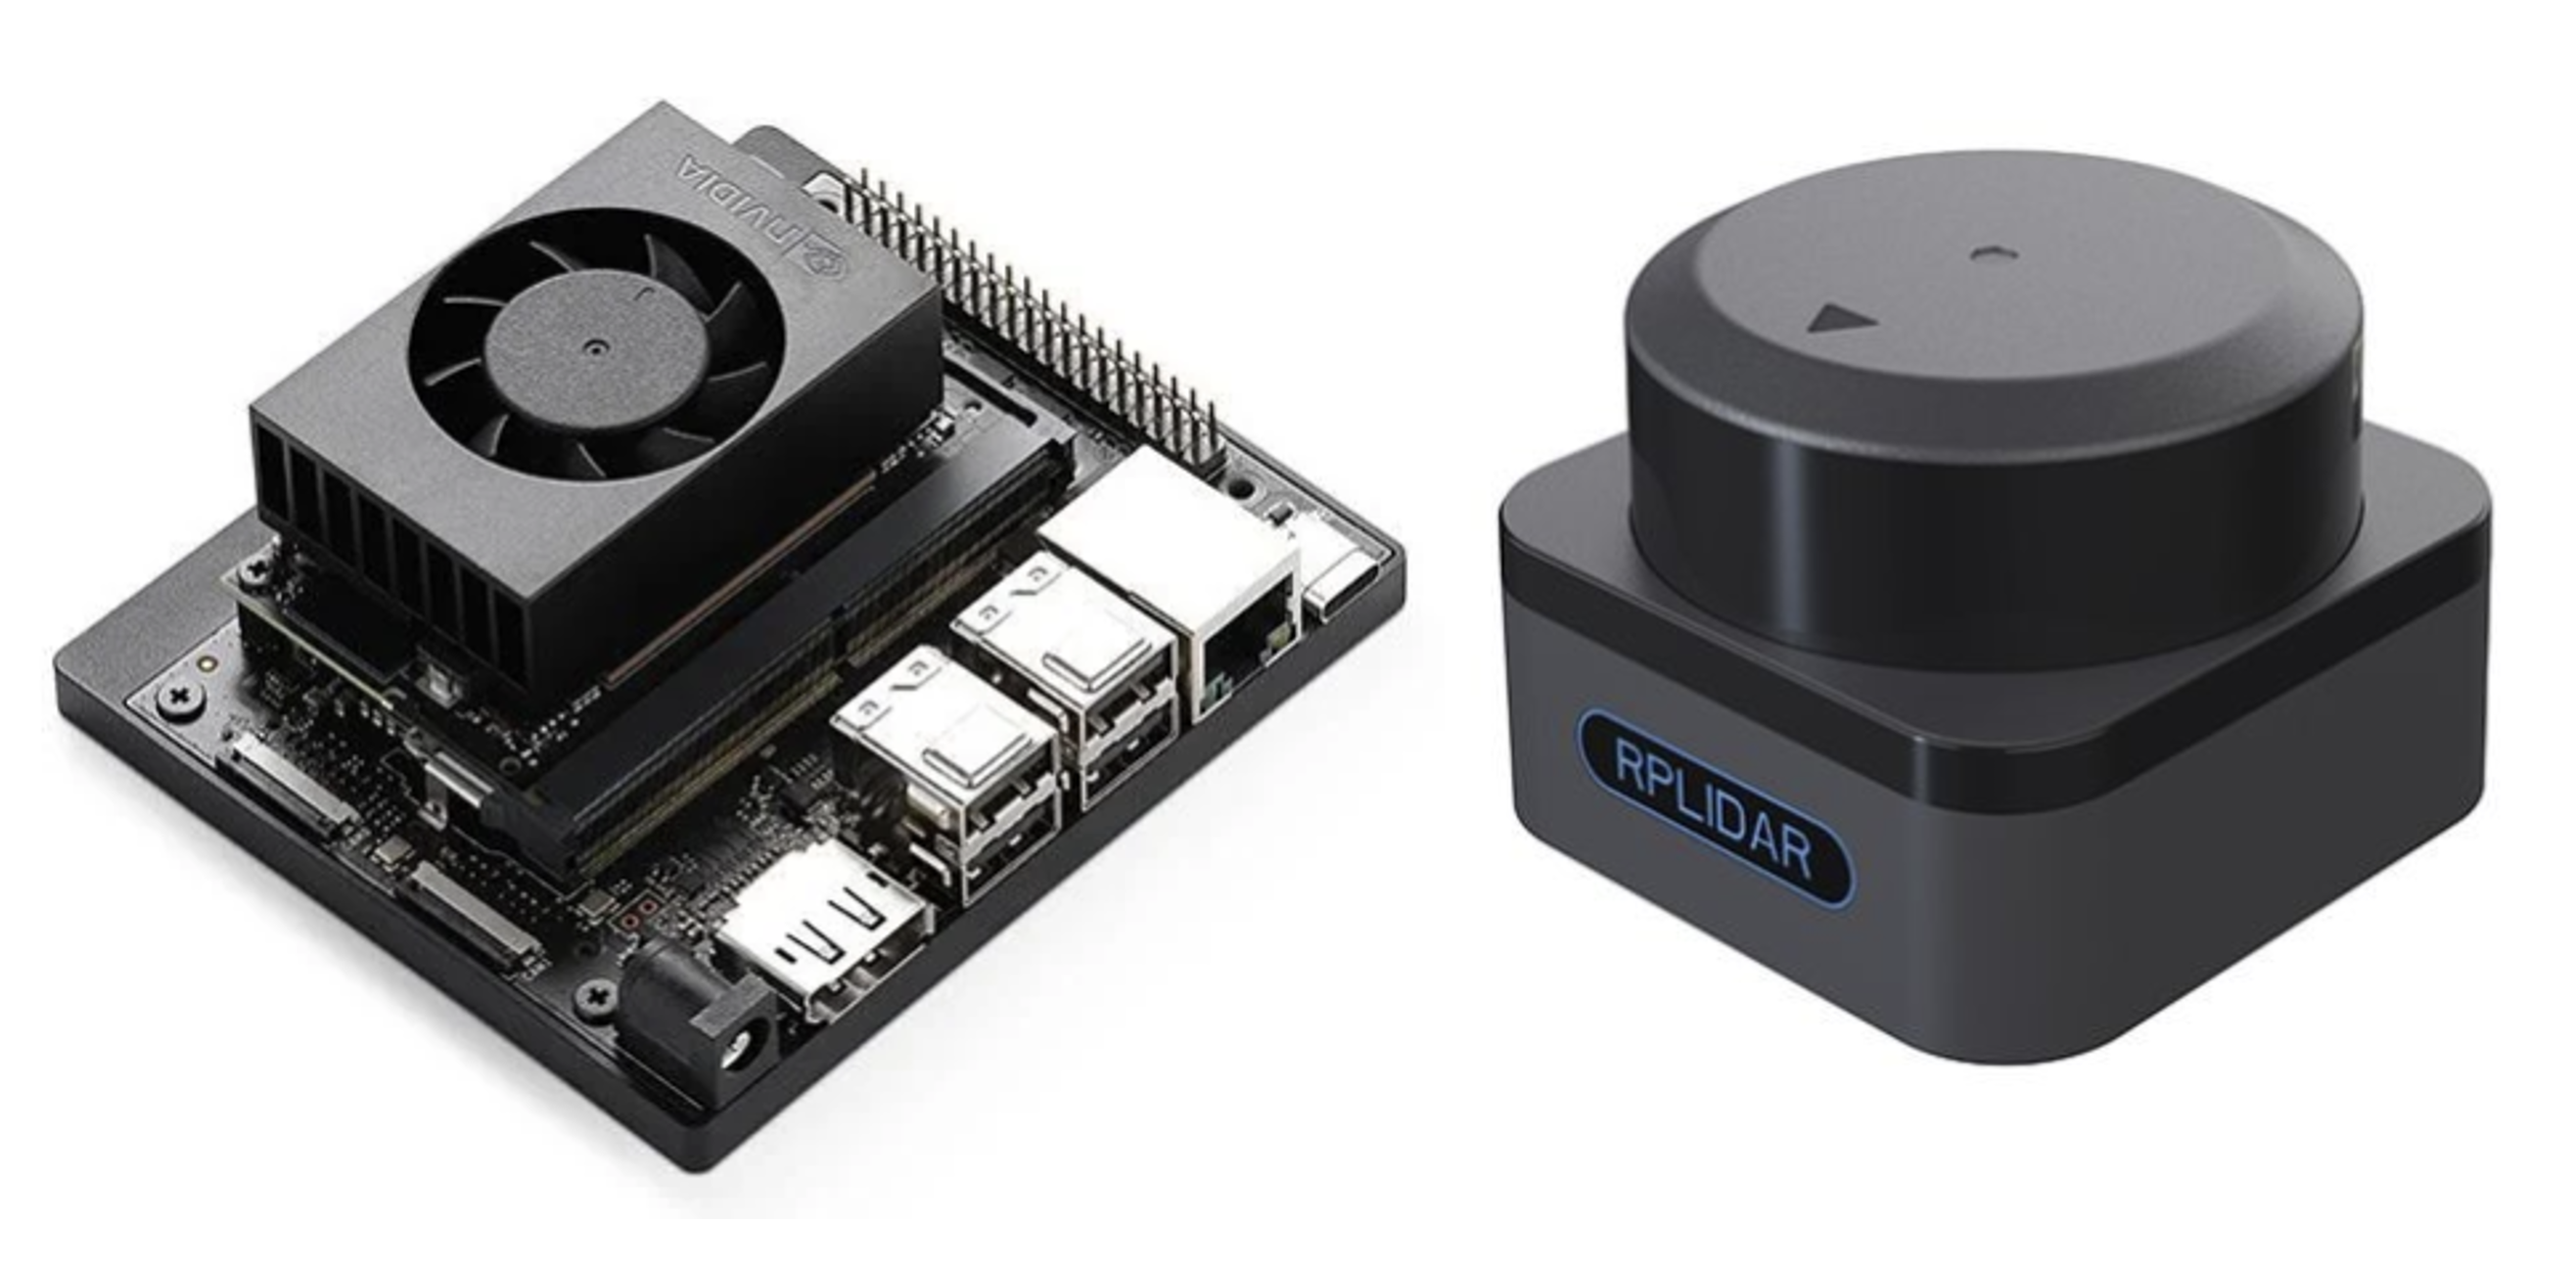
\includegraphics[width=0.5\linewidth]{assets/images/hardware/JetsonNano+RPLiDAR.png}
    \caption{Image of the Jetson Nano Orin(left) and RPLiDAR S3 360(right)}
    \label{fig:enter-label}
\end{figure}
\paragraph*{}
The next step, after achieving closed-loop control using XDrive with ODrive firmware, is to purchase additional motor drivers and control all four wheels. This will allow us to properly drive the X-Drive omnidirectional system using the Jetson Nano (see \ref{fig:hardware-arch})), which will then be abstracted to operate under ROS.
\begin{figure}
    \centering
    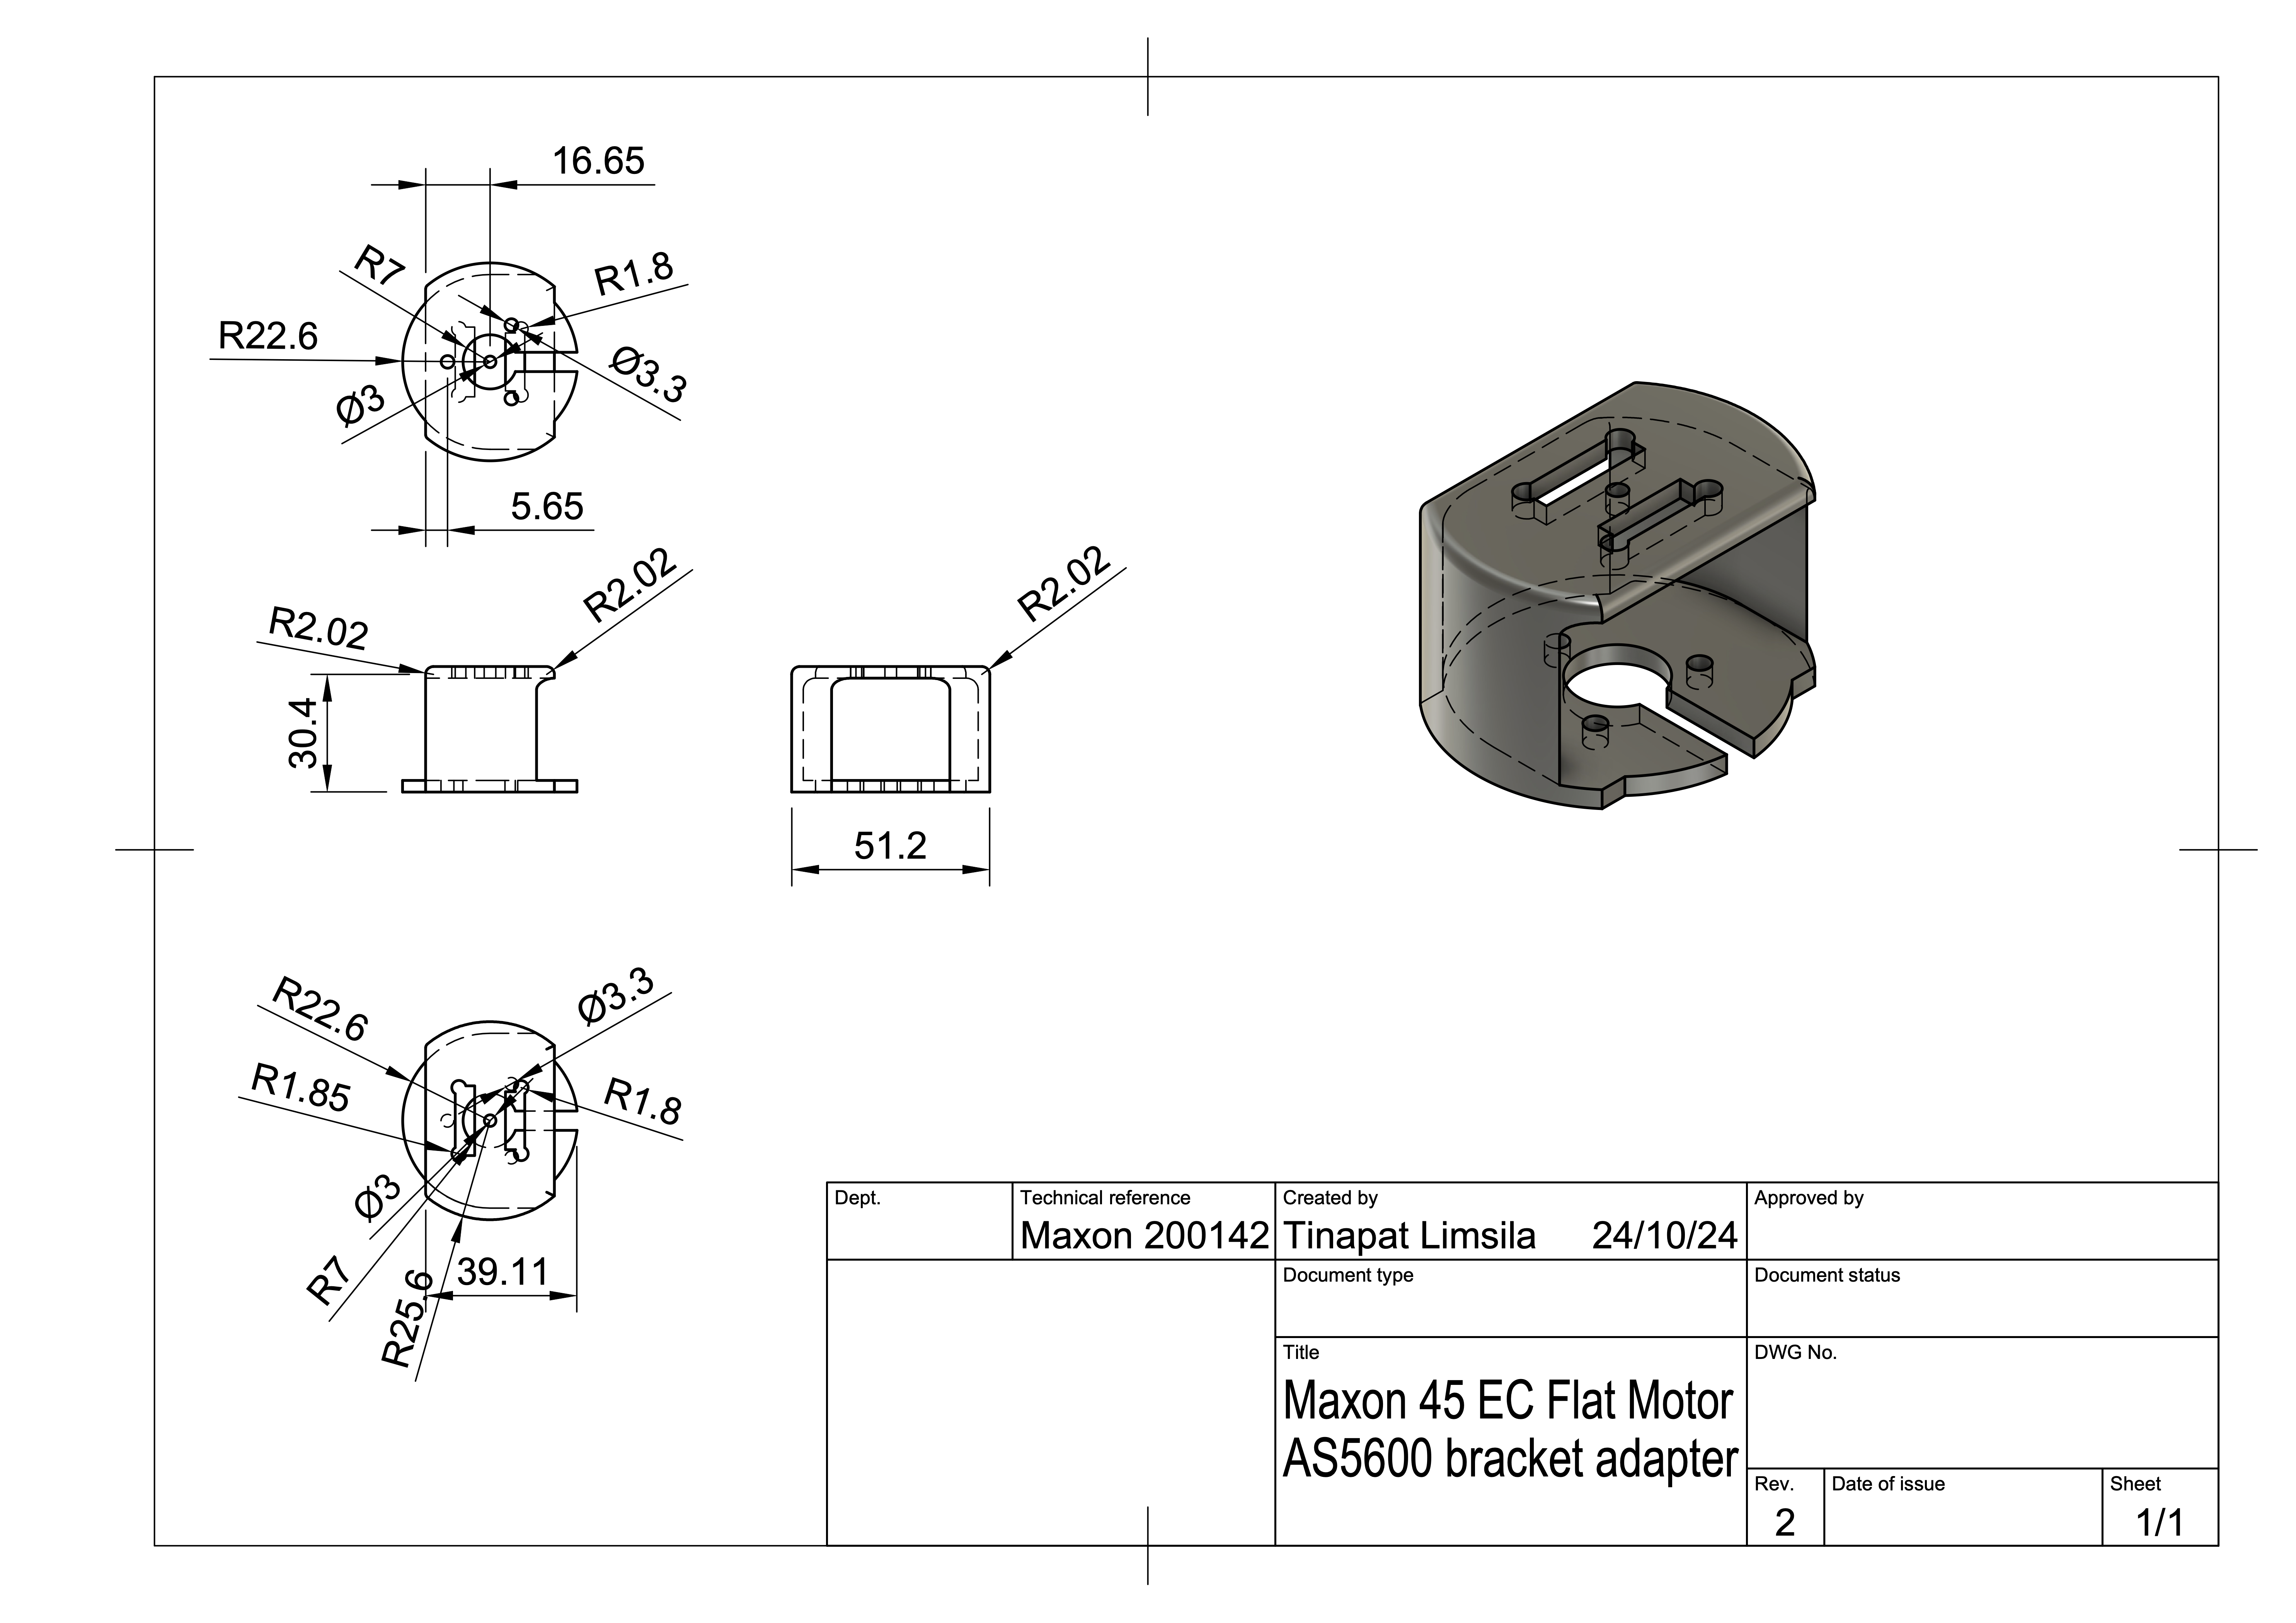
\includegraphics[width=1\linewidth]{assets/images/hardware/Maxon 45 EC Flat Motor AS5600 bracket adapter Drawing v1.png}
    \caption{CAD drawing of the bracket for the Maxon 45 EC Flat motor and the Magnetic Encoder for AS5600}
    \label{fig:real-single-robot}
\end{figure}

\begin{figure}
    \centering
    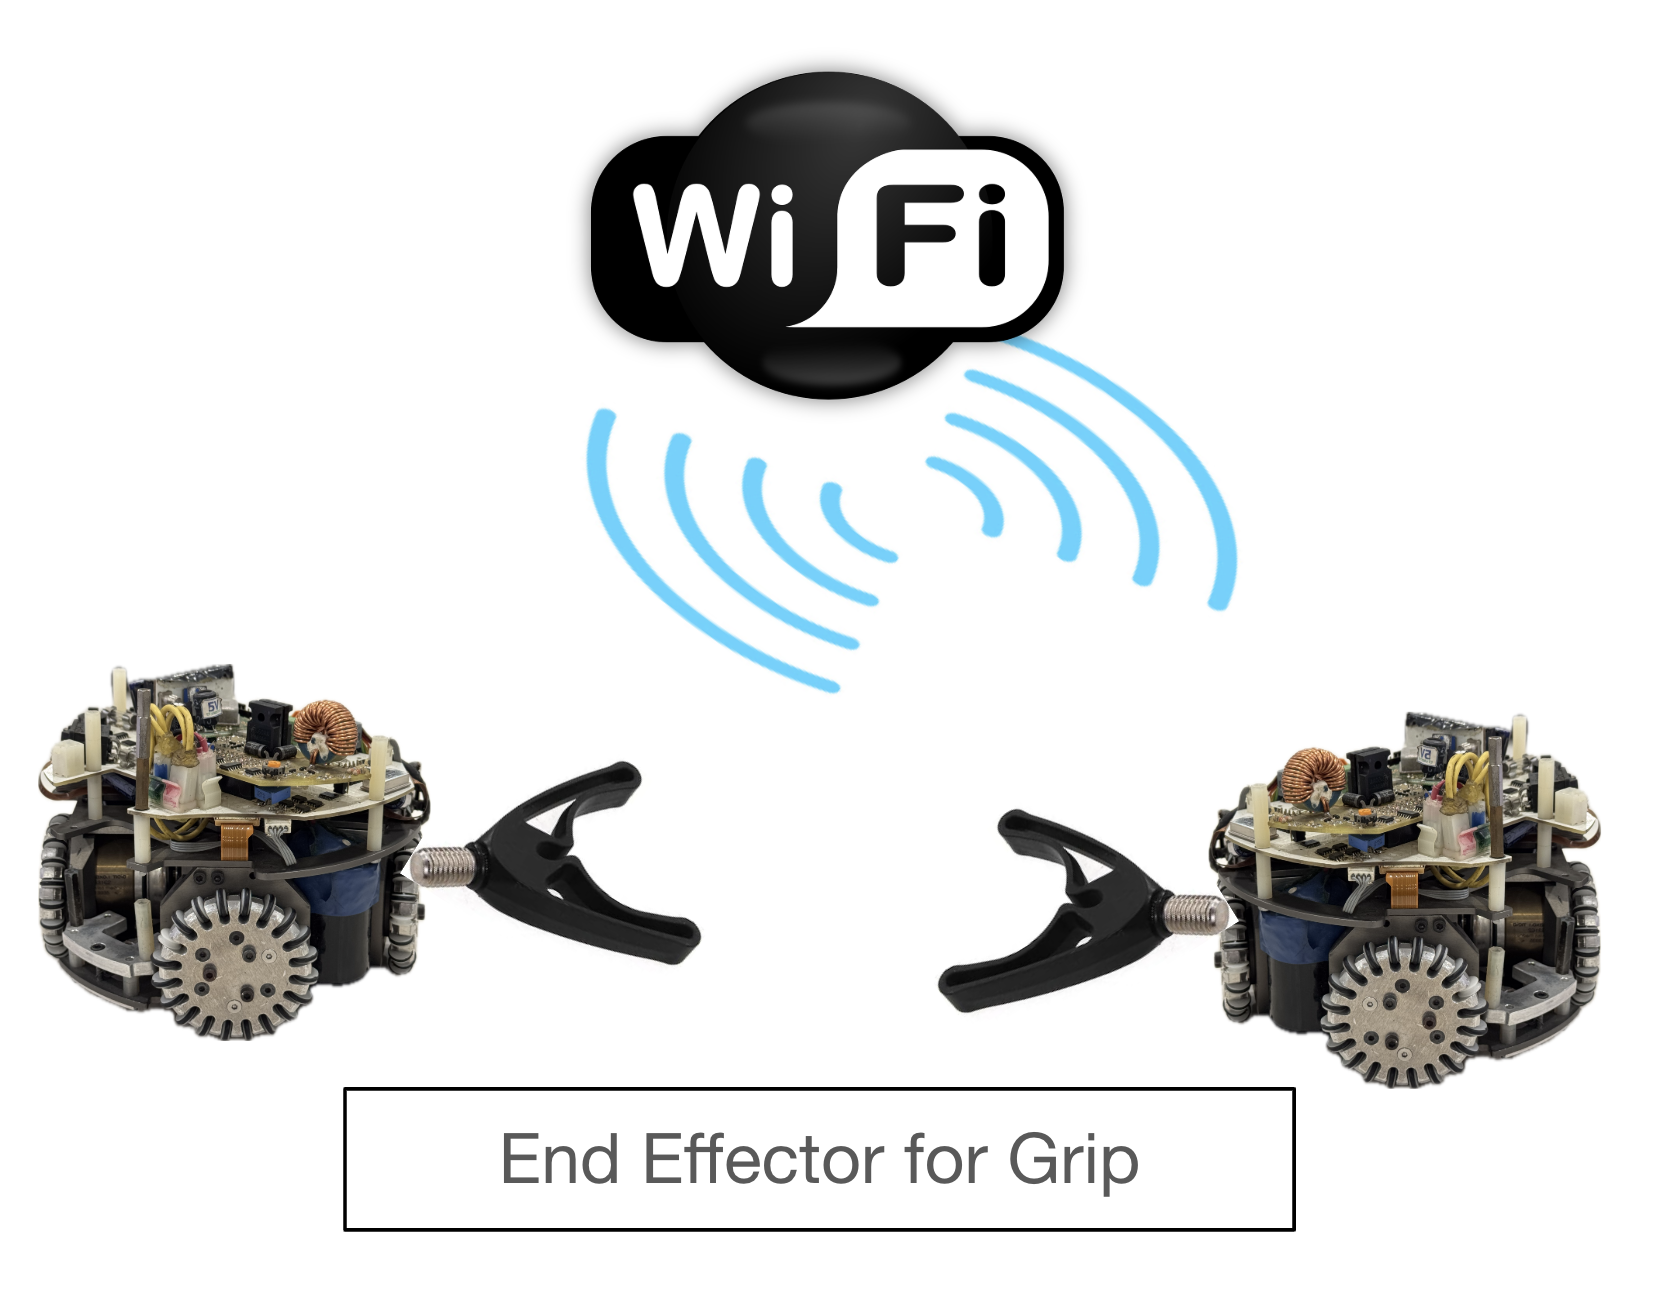
\includegraphics[width=0.5\linewidth]{assets/images/hardware/endeffector.png}
    \caption{Image of the two swarm robot with end effectors with communication via WiFi}
    \label{fig:effector-2-robot}
\end{figure}
\begin{figure}
    \centering
    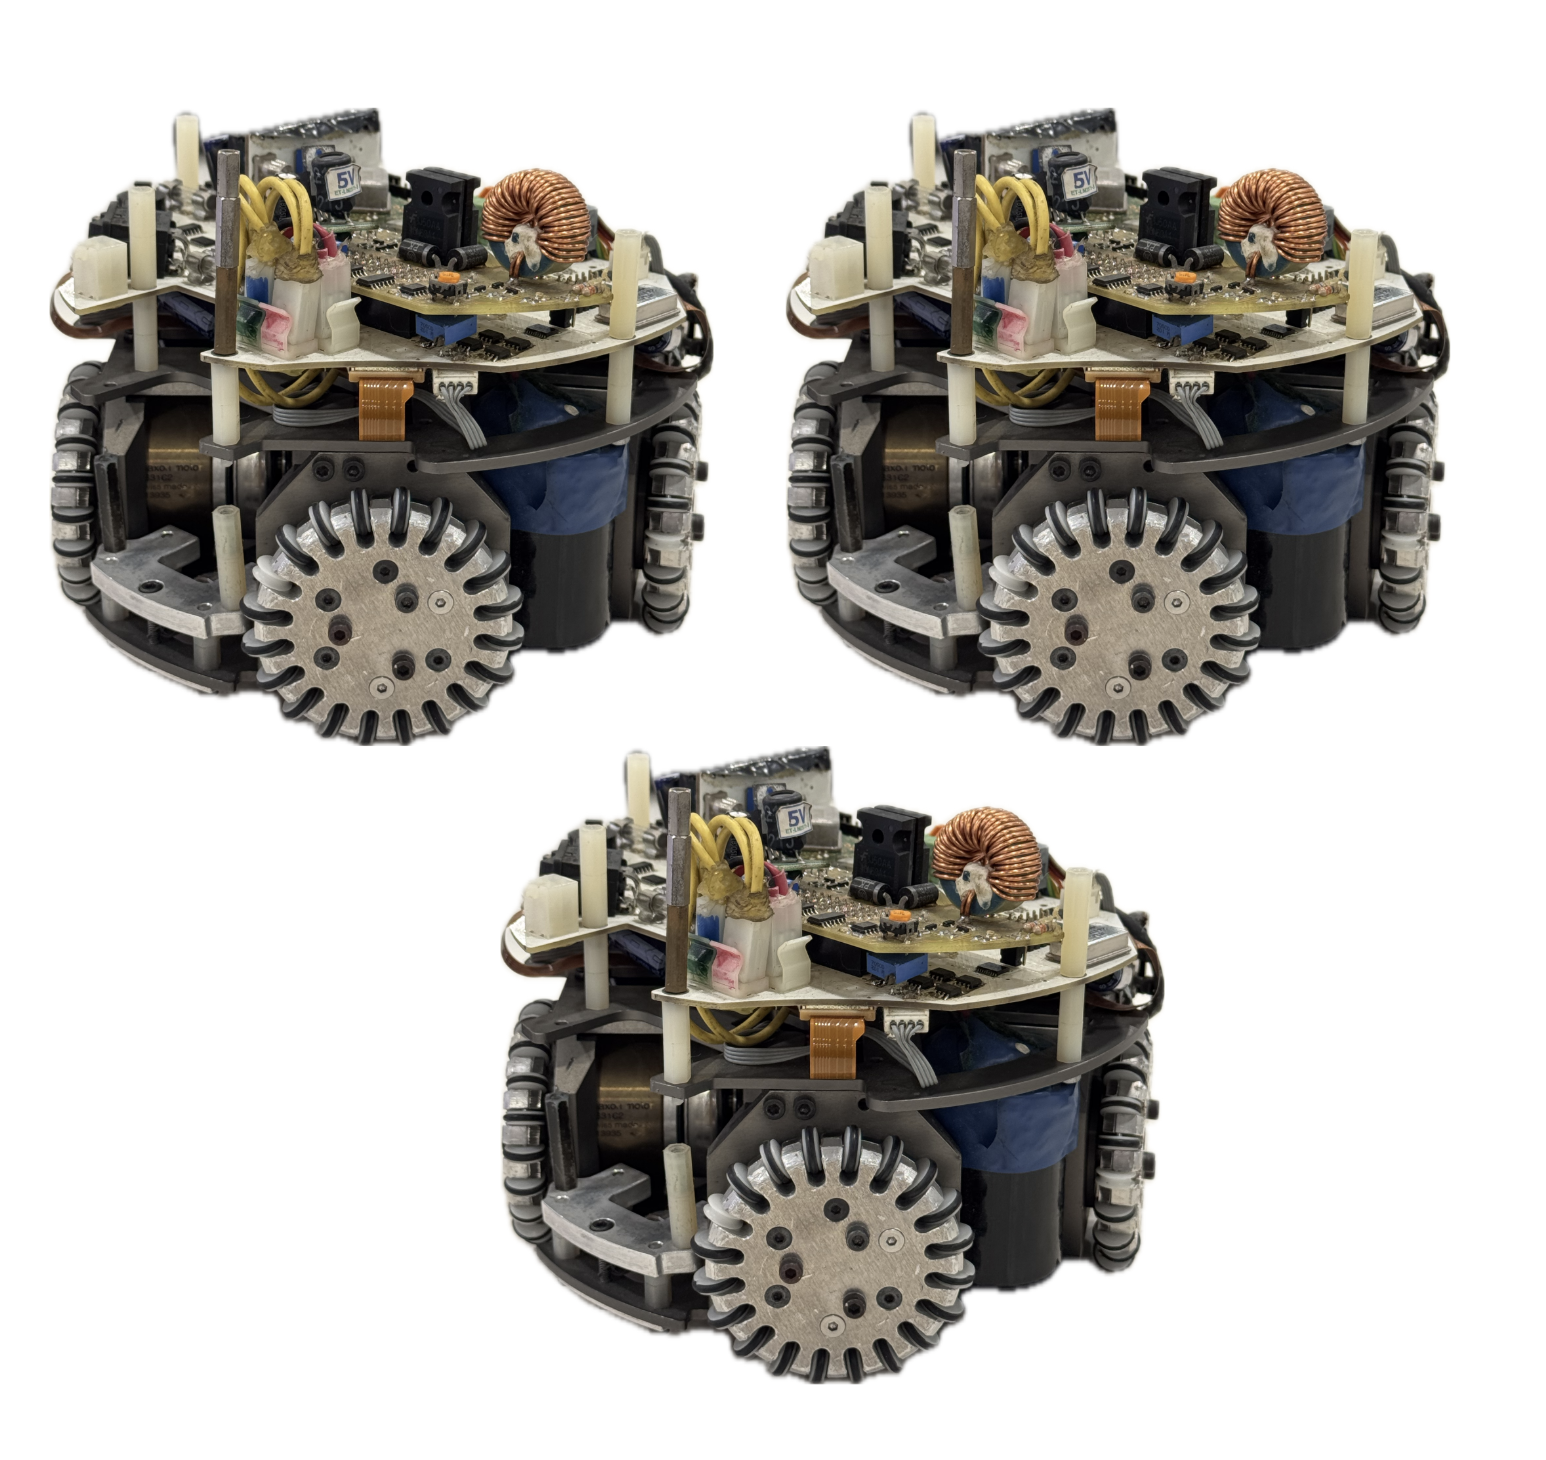
\includegraphics[width=0.5\linewidth]{assets/images/hardware/3swarmrobots.png}
    \caption{Image of the 3 acquired swarm robot pre-modification}
    \label{fig:3-robot}
\end{figure}\begin{figure}
    \centering
    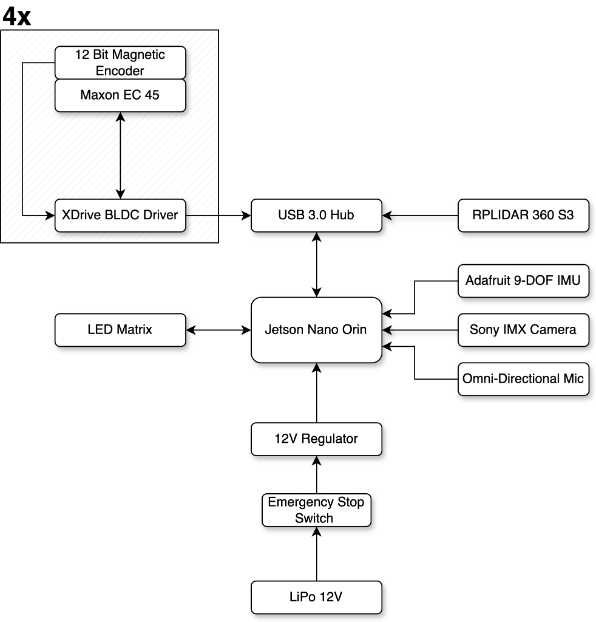
\includegraphics[width=0.75\linewidth]{assets/images/hardware/hardware-architecture.png}
    \caption{Image of a the hardware architecture and I/O of the system}
    \label{fig:hardware-arch}
\end{figure}

Our hardware in Figure \ref{fig:hardware-arch}, will have safety features such as microphones and an emergency stop button if the robot has software malfunctions. The LED matrix will be the indicator for taskmaster. RPLiDAR 360 S3 will be used for Graph SLAM with the ROS interface package provided. 
